\chapter{Conceptos previos}

\section{Procesamiento Lenguaje Natural}
\label{chap:pln}

\subsection{Introducción al Procesamiento del Lenguaje Natural}

El \acrfull{pln} es la rama de la \gls{ia} encargada de la interacción entre computadoras y el lenguaje humano. Este campo integra la lingüística computacional, basada en el modelado de reglas del lenguaje, con modelos estadísticos y algoritmos de aprendizaje profundo (\gls{dl}) y aprendizaje automático (\gls{ml}) \cite{stryker_what_nlp}.

El \gls{pln} forma parte a día de hoy de muchos motores de búsqueda, chatbots para atención al cliente (ya sea por escrito o por voz), y asistentes digitales como Alexa de Amazon o Siri de Apple.

El campo de la computación lingüística incluye tradicionalmente diversas fases para el análisis. Para el análisis de las palabras existen dos enfoques principales:

\begin{itemize}
      \item \textbf{Análisis de dependencias:} Examina las relaciones gramaticales binarias entre las palabras, identificando, por ejemplo, qué palabra modifica a cuál o cuál es el sujeto y el verbo principal.

      \item \textbf{Análisis de constituyentes:} Construye un árbol sintáctico que representa la estructura gramatical anidada de una oración, descomponiéndola en sintagmas o frases ordenadas jerárquicamente.
\end{itemize}

\subsection{Fases del \glsentryshort{pln}}

Las fases para realizar el \gls{pln} se pueden observar en la Figura \ref{fig:FasesNLP}:

\begin{figure}[h]
      \centering
      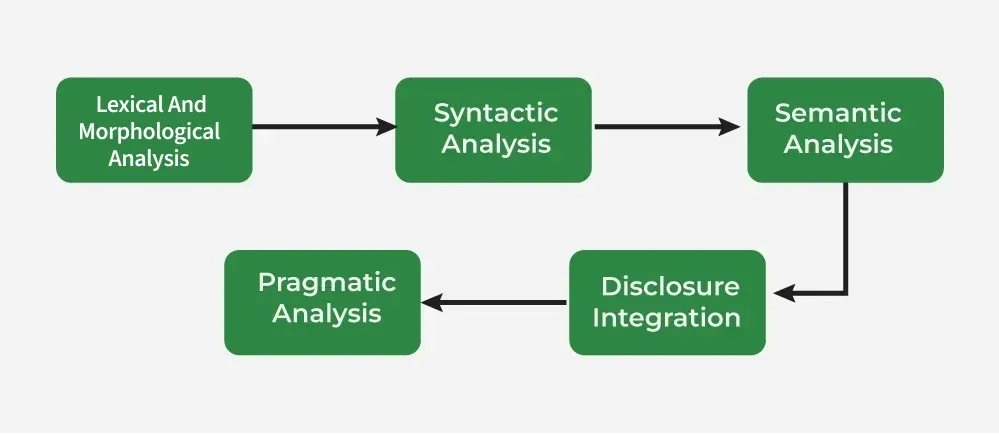
\includegraphics[width=1.0\linewidth]{imagenes/FasesNLP.png}
      \caption{Esquema de las fases del \gls{pln}. Extraído de \cite{geeksforgeeks_phases_nlp_2025}.}
      \label{fig:FasesNLP}
\end{figure}

A continuación, basándose en la estructura descrita en \cite{geeksforgeeks_phases_nlp_2025}, se detalla en qué consiste cada una de estas fases:

\subsubsection{Preprocesamiento y Tokenización}

Esta fase constituye el nivel inicial del procesamiento lingüístico computacional. Su propósito fundamental es transformar el texto crudo en una secuencia estructurada de unidades discretas y manejables. Para lograrlo, se integran diversas tareas de análisis léxico y morfológico que preparan la información para las etapas posteriores.

\begin{enumerate}
      \item \textbf{Preprocesamiento:} Esta fase inicial comprende un conjunto de operaciones destinadas a homogeneizar el texto. Entre las principales subtareas se encuentran la limpieza del contenido, la normalización (como la conversión a minúsculas) y la eliminación de caracteres especiales. Adicionalmente, suele llevarse a cabo la supresión de las \textit{stopwords}, que son palabras de muy alta frecuencia pero que carecen de una gran carga semántica (tales como ``el'', ``de'', ``y''). Como parte de este preprocesamiento, también se aplican técnicas de análisis morfológico para estandarizar el vocabulario:
            \begin{itemize}
                  \item \textit{Lematización:} Consiste en convertir las palabras a su forma base o lema canónico (por ejemplo, el verbo ``soy'' se transforma en ``ser'').
                  \item \textit{Stemming:} Se basa en reducir las palabras a su raíz léxica, eliminando sufijos y prefijos (por ejemplo, ``niñero'' se reduce a ``niño'').
            \end{itemize}

      \item \textbf{Tokenización:} Representa el proceso crítico mediante el cual se segmenta el flujo de texto en unidades atómicas significativas, denominadas \textit{tokens}.

            A modo de ejemplo, la oración \textit{Me gusta programar} se dividiría en la siguiente lista de tokens: \texttt{[``Me'', ``gusta'', ``programar'']}.

            La granularidad de los tokens depende del modelo empleado. Pueden corresponder a palabras completas, subpalabras (una técnica común en los modelos de tipo \gls{gpt}) o incluso a caracteres individuales. Una vez completada la tokenización, a cada token se le asigna un índice numérico único dentro de un vocabulario, un paso indispensable para la posterior generación de representaciones vectoriales o \textit{Embeddings} (concepto que se desarrollará en detalle en el Capítulo \ref{chap:word_embeddings}).

      \item \textbf{Etiquetado gramatical (\gls{pos} Tagging):} En esta etapa se asigna a cada token su correspondiente categoría morfológica (como sustantivo, verbo, adjetivo, entre otras), tomando en consideración tanto su definición formal como el contexto en el que aparece. Esto resulta esencial para desambiguar la función sintáctica que desempeña cada palabra en la oración.

            Siguiendo con el ejemplo anterior, el etiquetado de los tokens daría como resultado: \texttt{[``Me'' $\rightarrow$ Pronombre, ``gusta'' $\rightarrow$ Verbo, ``programar'' $\rightarrow$ Verbo]}.
\end{enumerate}

\subsubsection{Análisis sintáctico}

El análisis sintáctico examina la organización de las palabras dentro de una oración para verificar que se cumple con las reglas gramaticales del idioma. El objetivo fundamental de esta fase es la generación de un \textbf{árbol de análisis sintáctico}, el cual representa jerárquicamente la estructura gramatical del texto analizado. Esta representación estructurada permite a los sistemas computacionales interpretar las relaciones de dependencia y jerarquía entre los distintos elementos léxicos. Las tareas principales que abarca son:

\begin{itemize}
      \item \textbf{Etiquetado gramatical:} Se fundamenta en el proceso de \gls{pos} Tagging explicado en la fase de \textit{Preprocesamiento y Tokenización}. En esta etapa de análisis sintáctico, las categorías morfológicas previamente asignadas a cada token se utilizan para validar la corrección de la estructura jerárquica de la oración.
      \item \textbf{Resolución de ambigüedad sintáctica:} Consiste en determinar la estructura gramatical correcta cuando una oración puede analizarse de múltiples formas. Por ejemplo, en la frase \textit{Vi al hombre con el telescopio}, el sistema debe resolver si el telescopio es el instrumento utilizado por el sujeto para ver, o si es un objeto que lleva consigo el hombre.
\end{itemize}

\subsubsection{Análisis semántico}

Esta fase se centra en la coherencia lógica y la relevancia contextual del enunciado. Su objetivo principal es interpretar el significado de las palabras, analizando tanto su definición de diccionario como su variación según el contexto de uso. De este modo, se busca comprender el rol semántico de cada palabra para construir una representación lógica del mensaje. Las tareas fundamentales que abarca esta fase son:

\begin{enumerate}
      \item \textbf{\gls{ner}:} Se ocupa de la identificación y clasificación de elementos clave en el texto, tales como nombres de personas, ubicaciones geográficas, organizaciones, etc.
            \\
            Ejemplo: En la oración \textit{Mercedes anunció un nuevo coche en Berlín}, el sistema \gls{ner} identificaría a \textit{Mercedes} como una \textit{Organización} y a \textit{Berlín} como un \textit{Lugar}.

      \item \textbf{\gls{wsd}:} Consiste en identificar el significado exacto de una palabra polisémica basándose en el contexto en el que se encuentra (proceso conocido como resolución de ambigüedad léxico-semántica).
            \\
            Ejemplo: El término \textit{banco} se interpreta como una \textit{entidad financiera} en la frase \textit{Fui a sacar dinero al banco}, pero adquiere el significado de \textit{asiento} en la oración \textit{Me senté en el banco del parque}.
\end{enumerate}

\subsubsection{Integración del discurso}

Este proceso analiza cómo las oraciones individuales se conectan y relacionan entre sí para entender el contexto global. El objetivo de esta fase es garantizar que el significado del texto mantenga su coherencia lógica a través de los distintos párrafos y frases. Los aspectos fundamentales de esta fase son:

\begin{itemize}
      \item \textbf{Resolución de anáforas:} Consiste en identificar la conexión entre un pronombre y lo mencionado previamente en el texto.
            \\
            Ejemplo: En la secuencia \textit{Esther fue a comprar. Ella compró fruta}, el sistema debe vincular el pronombre \textit{Ella} con \textit{Esther}.

      \item \textbf{Referencias contextuales:} Aborda la interpretación de palabras o expresiones cuyo significado completo depende intrínsecamente de la información proporcionada en oraciones anteriores o posteriores.
            \\
            Ejemplo: La frase \textit{Fue un buen día} adquiere un significado concreto únicamente si se analiza dentro del contexto de la conversación.
\end{itemize}

\subsubsection{Análisis pragmático}

Esta fase final analiza más allá de la interpretación literal de las oraciones para inferir el significado real que se pretende transmitir. A diferencia del análisis semántico, que se ocupa del significado proposicional de las palabras, el análisis pragmático examina factores como el tono y el contexto. Las tareas principales de esta fase son:

\begin{itemize}
      \item \textbf{Detección de intenciones:} El sistema debe ver el propósito de la comunicación (si es una petición, una queja, una orden, etc.).
            \\
            Ejemplo: Ante la pregunta \textit{¿Tienes hora?}, el análisis pragmático entiende que la intención real del usuario es saber qué hora es, no una pregunta de sí o no.

      \item \textbf{Interpretación de lenguaje figurado:} Se encarga de identificar metáforas, ironías o frases hechas.
            \\
            Ejemplo: En la expresión \textit{Echar una mano}, el análisis pragmático entiende que significa \textit{ayudar a alguien}.
\end{itemize}


\section{Computación cuántica}

\subsection{Números complejos}
\label{chap:numeros_complejos}

El conjunto de los números complejos, representado por el símbolo $\mathbb{C}$, es la combinación de números reales e imaginarios \cite{ferrovial_numeros_complejos}. La parte real se puede expresar por un número entero o sus decimales, la parte imaginaria es aquella cuyo cuadrado es negativo.


Los números complejos sirven para dar sentido a la raíz cuadrada de números negativos. Esto permite que ecuaciones de segundo grado con discriminante negativo, puedan ser resueltas. Con esto se abre la puerta a un gran mundo en el que todas las operaciones (excepto dividir entre 0), son posibles.


Las características principales de los números complejos con las siguientes:

\begin{itemize}
    \item Tiene distintas formas de expresarse.
    \item Dos números complejos se consideran iguales cuando tienen mismo componente real e imaginario.
    \item $\mathbb{C}$ conforma un espacio vectorial de dos dimensiones: la de los números reales y la de los imaginarios.
    \item Los números complejos no pueden mantener un orden. Es decir no se puede encontrar una propiedad $>$ o $<$ que un número para todos los números complejos.
\end{itemize}

\subsubsection{Representación binómica}

Un número complejo puede expresarse de forma puramente algebraica mediante su \textbf{representación binómica}. Esta forma divide el número en la suma de dos componentes:

\[
    z = a + bi, \quad a, b \in \mathbb{R}, \quad i = \sqrt{-1};
\]

Con esta representación matemática, $a$ constituye la \textbf{parte real} y $b$ la \textbf{parte imaginaria} del número complejo. Si un número carece de parte real ($a=0$), se le denomina imaginario puro.

A partir de la representación binómica de un número complejo se pueden definir a su vez otros dos números complejos fuertemente relacionados:

\begin{itemize}
    \item \textbf{Conjugado:} Se define cambiando el signo de la parte imaginaria, denotándose como $\overline{z} = a - ib$.
    \item \textbf{Inverso:} Se define como $z^{-1} = \frac{a}{a^2 + b^2} - \frac{b}{a^2 + b^2}i$.
\end{itemize}

Al estar expresados en forma binómica, las operaciones aritméticas básicas entre dos números complejos $z_1 = a + bi$ y $z_2 = c + di$ se realizan aplicando las propiedades algebraicas de los números reales y teniendo en cuenta que $i^2 = -1$:

\begin{itemize}
    \item \textbf{Suma y resta:} Se operan las partes reales e imaginarias por separado. Es decir, $z_1 \pm z_2 = (a \pm c) + (b \pm d)i$.
    \item \textbf{Multiplicación:} Se aplica la propiedad distributiva convencional y se simplifica, obteniendo $z_1 \cdot z_2 = (ac - bd) + (ad + bc)i$.
    \item \textbf{División:} Para realizar $\frac{z_1}{z_2}$, se multiplica tanto el numerador como el denominador por el conjugado del denominador ($\overline{z_2}$). Esto elimina la parte imaginaria del divisor, permitiendo separar el resultado final en parte real e imaginaria.
\end{itemize}

\subsubsection{Representación geométrica en $\mathbb{R}^2$}

Debido a que la forma binómica de un número complejo $z = a + bi$ está unívocamente definida por dos valores reales ($a$ y $b$), existe una correspondencia natural con el espacio bidimensional $\mathbb{R}^2$. Por ello, para representar gráficamente un número complejo, se utiliza un sistema de coordenadas cartesiano denominado \textbf{plano complejo} o plano de Argand \cite{sangaku_representacion_complejos}.

Este plano está formado por dos ejes perpendiculares: un \textbf{eje real} (horizontal) donde se ubica la parte real $a$, y un \textbf{eje imaginario} (vertical) donde se posiciona la parte imaginaria $b$. De este modo, el número complejo puede representarse como el punto $(a,b)$ en dicho plano. A este punto geométrico se le conoce formalmente como el \textbf{afijo} del número complejo.

La Figura \ref{fig:PlanoComplejo} muestra cómo este punto se posiciona en el plano en base a sus componentes.

\begin{figure}
    \centering
    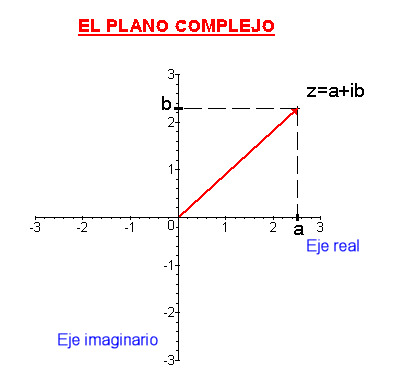
\includegraphics[width=0.5\linewidth]{imagenes/PlanoComplejoRepreGeometrica.jpg}
    \caption{Plano sobre como representar número complejo}
    \label{fig:PlanoComplejo}
\end{figure}

Basándonos en la definición del apartado anterior sobre el inverso y conjugado de un número complejo, al representarlo de forma gráfica queda de la siguiente manera:

\begin{figure}
    \centering
    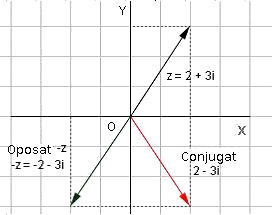
\includegraphics[width=0.5\linewidth]{imagenes/ConjInvCompPlano.jpg}
    \caption{Representación en plano sobre conjugado e inverso}
    \label{fig:ConjInversoPlanoComp}
\end{figure}

\subsubsection{Representación forma polar}

Esta representación sirve para destacar los atributos gráficos que tienen los números complejos. Se basa en 2 conceptos fundamentales:

\begin{itemize}
    \item \textbf{Módulo ($r$):} Distancia Euclidiana del afijo al origen de coordenadas, calculada como $r = |z| = \sqrt{a^2 + b^2}$.
    \item \textbf{Argumento ($\alpha$ o $\arg(z)$):} Ángulo que forma el segmento $\overline{OZ}$ con el semieje real positivo, se obtiene mediante $\alpha = \arctan\left(\frac{b}{a}\right)$.
\end{itemize}

En la Figura \ref{fig:formaPolar} se puede apreciar visualmente esta representación en el plano.

\begin{figure}[h]
    \centering
    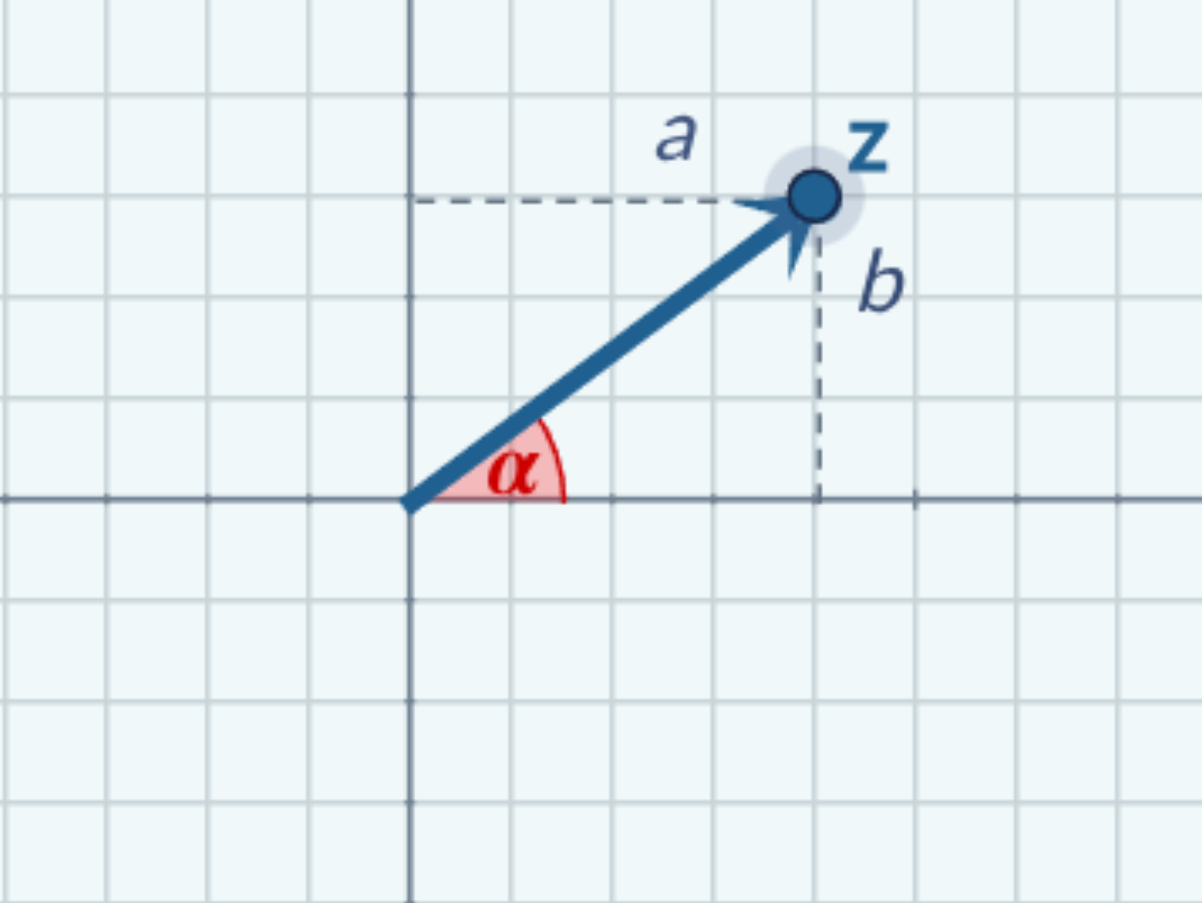
\includegraphics[height=5cm]{imagenes/FormaPolarNumComp.png}
    \caption{Gráfica de la forma polar de un número complejo}
    \label{fig:formaPolar}
\end{figure}

Utilizando estos dos parámetros, el número complejo $z$ se puede expresar de una forma más compacta, conocida como \textbf{forma polar}, la cual se denota matemáticamente como:

\[
    z = r_{\alpha};
\]

En base a la forma polar, se puede expresar $z$ en \textbf{forma trigonométrica} de la siguiente manera:

\[
    z = r (\cos \alpha + i \, \sen \alpha);
\]

Esta expresión permite la conversión de un número de su forma polar a su forma binómica ($z = a + bi$). Al distribuir el producto, se extrae explícitamente la correspondencia para cada una de las componentes cartesianas:

\begin{itemize}
    \item \textbf{Parte real:} $a = r \cos \alpha$
    \item \textbf{Parte imaginaria:} $b = r \sen \alpha$
\end{itemize}

\paragraph{Operaciones}

La forma polar (y su equivalente trigonométrica) simplifica enormemente las operaciones de multiplicación y división. Para demostrarlo, consideremos dos números complejos cualesquiera explícitamente definidos en su \textbf{forma trigonométrica}: $z_1 = r (\cos \alpha + i \sen \alpha)$ y $z_2 = r' (\cos \beta + i \sen \beta)$.

Al operar con ellos matemáticamente, se obtienen los siguientes resultados:

\begin{itemize}
    \item \textbf{Producto:} $z_1 \cdot z_2 = r \cdot r' \, (\cos(\alpha + \beta) + i \, \sen(\alpha + \beta))$\\
          Se observa que el módulo del número complejo resultante es el producto de los módulos iniciales ($r \cdot r'$), y su argumento es la suma de los argumentos ($\alpha + \beta$).

    \item \textbf{Cociente:} $\frac{z_1}{z_2} = \frac{r}{r'} \, (\cos(\alpha - \beta) + i \, \sen(\alpha - \beta))$\\
          El resultado del cociente es un número cuyo módulo es el cociente de los módulos ($\frac{r}{r'}$) y su argumento es la diferencia de los argumentos ($\alpha - \beta$).
\end{itemize}

Por lo que en \textbf{forma polar} quedaría de la siguiente manera:

\begin{itemize}
    \item \textbf{Producto:} $r_\alpha \cdot r_\beta' = (r \cdot r')_{\alpha+\beta}$
    \item \textbf{Cociente:} $\frac{r_\alpha}{r_\beta'} = \left(\frac{r}{r'}\right)_{\alpha - \beta}$
\end{itemize}

Para calcular \textbf{potencia} con exponente natural \textbf{n}, en forma polar, hay que elevar el módulo a \textbf{n} y multiplicar el argumento por \textbf{n}.

\[
    \left( r_\alpha \right)^n = \left( r^n \right)_{n \cdot \alpha};
\]

La \textbf{raíz n-esima} de un número complejo en forma polar, es otro número complejo \textbf{$m_\beta$} que debe de cumplir:

\[
    \left( m_\beta \right)^n = r_\alpha;
\]
\[
    m = \sqrt[n]{r} \quad \text{ y } \quad \beta = \frac{\alpha + \ang{360} \cdot k}{n} \quad \text{donde } k = 0, 1, 2, \dots, n-1;
\]

Todo número complejo tiene n raíces n-ésimas. Todos los afíjos están situados sobre una circunferencia y son los vértices de un polígono regular de n lados. \\

Un ejemplo de forma gráfica calculando la raíz n-esima con lo explicado anteriormente, es el que se ve en la Figura \ref{fig:Raiz3esimaComplejo}

\newpage
\begin{figure}[h]
    \centering
    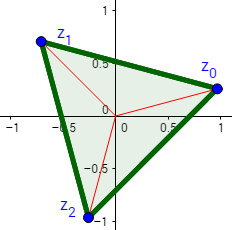
\includegraphics[height=5cm]{imagenes/Raiz3EsimaComplejoPolar.png}
    \caption{Raíz 3-esima del número complejo $z = i + 1$}
    \label{fig:Raiz3esimaComplejo}
\end{figure}

\subsubsection{Representación en forma exponencial}

Además de las representaciones binómica y polar, existe una tercera forma de expresar un número complejo que resulta de vital importancia en campos como la física y la computación cuántica. Gracias a la célebre \textbf{fórmula de Euler} \cite{pierce_formula_euler_2024}, se establece una equivalencia matemática directa entre las funciones trigonométricas y la función exponencial compleja:

\[
    e^{i\alpha} = \cos \alpha + i \, \sen \alpha;
\]

Si sustituimos esta identidad en la forma trigonométrica que vimos anteriormente ($z = r (\cos \alpha + i \, \sen \alpha)$), obtenemos la \textbf{forma exponencial} del número complejo:

\[
    z = r e^{i\alpha};
\]

Esta notación es extremadamente útil y será empleada junto con la notación de Dirac en la formulación de estados y operaciones cuánticas a lo largo de este trabajo, ya que simplifica de manera notable la representación algebraica de las rotaciones de fase y las operaciones matemáticas complejas.

\subsubsection{Notación Dirac (Bra-Ket)}
\label{sec:notacion_dirac}

La notación de Dirac nos da una manera de expresar estados en un espacio vectorial sin atarnos a un sistema de coordenadas específico, pero que hace muy sencillo elegir una base concreta y cambiar de una base a otra.

En esta notación \cite{pierce_braket_2025}, un \textbf{ket} representa los valores como un vector columna, mientras que un \textbf{bra} los representa como un vector fila.

\begin{itemize}
    \item \textbf{ket ($\ket{a}$):} Representa un vector columna cuyas componentes son números complejos. Si se tiene un vector $\vec{a} \in \mathbb{C}^n$, su representación en Dirac es el ket $\ket{a}$.
    \item \textbf{bra ($\bra{a}$):} Representa el vector fila resultante de aplicar el conjugado transpuesto al ket correspondiente. Matemáticamente, se denota como $\bra{a} = \ket{a}^{\dagger}$.
\end{itemize}

Por ejemplo, si consideramos un vector en el espacio bidimensional $\mathbb{C}^2$ con dos componentes complejas genéricas $\alpha$ y $\beta$, su representación en ket y su correspondiente bra serían:

\begin{itemize}
    \item \textbf{ket:} $\ket{\psi} = \begin{pmatrix} \alpha \\ \beta \end{pmatrix}$
    \item \textbf{bra:} $\bra{\psi} = \ket{\psi}^{\dagger} = \begin{pmatrix} \alpha^* & \beta^* \end{pmatrix}$
\end{itemize}

donde $\alpha^*$ y $\beta^*$ son los complejos conjugados de $\alpha$ y $\beta$. Otro ejemplo fundamental en computación cuántica es la base canónica en $\mathbb{C}^2$, la cual se representa con los kets $\ket{0}$ y $\ket{1}$:

\[
    \ket{0} = \begin{pmatrix} 1 \\ 0 \end{pmatrix}, \quad \ket{1} = \begin{pmatrix} 0 \\ 1 \end{pmatrix};
\]

Utilizando esta notación, se puede definir las siguientes operaciones:

\begin{itemize}
    \item \textbf{Producto interno:} Es un número obtenido al multiplicar un bra por un ket.
          \[ \braket{a|b} = \begin{pmatrix} a_1^{*} & a_2^{*} \end{pmatrix} \begin{pmatrix} b_1\\ b_2 \end{pmatrix} = a_1^{*} b_1 + a_2^{*} b_2 \]
    \item \textbf{Producto externo:} Resulta en una matriz, obtenida al multiplicar un ket por un bra. Si consideramos que los kets $\ket{e_i}$ forman una base ortonormal del espacio de Hilbert, el término $\ket{e_i}\bra{e_j}$ representa una matriz con un $1$ en la fila $i$ y la columna $j$ (y ceros en el resto). De este modo, cualquier matriz $\mathbf{A}$ se puede construir ponderando estas matrices base por sus respectivos coeficientes $A_{ij}$:
          \[ \mathbf{A} = \sum_{i,j=1}^{N} A_{ij}\,\ket{e_i}\bra{e_j} \]
\end{itemize}


\subsection{Qubits}
\label{chap:qubits}

Un \gls{qubit} es el análogo cuántico al bit clásico \cite{ionos_qubits_2023}. Mientras el bit tiene \textbf{dos posibles estados}, el 0 y el 1, el \gls{qubit} se representa como un vector en el espacio vectorial $\mathbb{C}^2$. La base del espacio más utilizada, se denomina base computacional y se corresponde con la base canónica de $\mathbb{C}^2$, que en \textit{notación de Dirac}, son los vectores $\ket{0}$ y $\ket{1}$:

\begin{equation*}
    \begin{array}{rl}
        \ket{0} = & \begin{bmatrix}
                        1 \\ 0
                    \end{bmatrix} \in \mathbb{C}^2 \\
        \ket{1} = & \begin{bmatrix}
                        0 \\ 1
                    \end{bmatrix}
    \end{array}
\end{equation*}

\textbf{Un estado cuántico} es la descripción matemática completa de un sistema cuántico aislado (en este caso, un \gls{qubit}). Más allá de ser un simple vector, este estado encapsula toda la información física y probabilística que podemos conocer del sistema antes de interactuar con él. Dado que se define dentro de un espacio de Hilbert, el estado cuántico obedece al \textit{principio de superposición}, lo que le confiere la capacidad de existir en múltiples configuraciones clásicas de forma simultánea hasta que se produce el colapso mediante una medición.

\subsubsection{Expresión del Qubit en Superposición}
Gracias al principio de superposición mencionado anteriormente, un qubit $\ket{\Psi}$ no tiene por qué estar exclusivamente en el estado $\ket{0}$ o en el estado $\ket{1}$. En su lugar, su estado puede ser una \textbf{combinación lineal} de ambos vectores base. A este comportamiento se le denomina \textbf{superposición cuántica}, y permite que el qubit exista como una mezcla simultánea de ambos estados clásicos. En notación de Dirac, esto se representa algebraicamente como:

\[
    \ket{\Psi} = \alpha_0\ket{0} + \alpha_1\ket{1};
\]

Donde $\alpha_0$ y $\alpha_1$ son las \textbf{amplitudes de probabilidad}. De forma general, estas amplitudes se definen como números complejos (lo que, por definición matemática, también incluye a los números reales como un caso particular). Dado que estos coeficientes pueden tomar infinitos valores continuos, un qubit puede adoptar \textbf{infinitos} estados posibles, frente a los únicos dos valores (0 y 1) de un bit clásico. Para que este estado sea válido físicamente, su norma debe ser unitaria, asegurando que la suma de las probabilidades sea 1:

\[
    |\alpha_0|^2 + |\alpha_1|^2 = 1;
\]

Cabe destacar que no existe una forma directa de determinar los valores exactos de $\alpha_0$ y $\alpha_1$, ya que el estado cuántico interno no es directamente observable. Antes de realizar una medición, el qubit se encuentra en esta superposición inestable de los estados $\ket{0}$ y $\ket{1}$.

Para conocer el resultado de una computación cuántica, es necesario medir los qubits \cite{sholtis_measure_qubits_2019}. Sin embargo, el acto de medición implica una interacción física que perturba irreversiblemente el sistema. Esto provoca que el qubit abandone su estado de superposición y experimente el \textbf{colapso}. Al colapsar, el qubit se ve forzado a tomar un único valor clásico definido, es decir, pasa a ser estrictamente un $0$ lógico (estado $\ket{0}$) o un $1$ lógico (estado $\ket{1}$). Una vez medido, el qubit se comporta como un bit clásico ordinario, y la información sobre sus amplitudes cuánticas originales se pierde de forma irrecuperable.

La probabilidad exacta de que el qubit colapse hacia un estado u otro está dictada por la \textbf{regla de Born}. Esta regla establece que la probabilidad de observar cada resultado clásico es igual al módulo al cuadrado de su amplitud correspondiente ($P(0) = |\alpha_0|^2$ y $P(1) = |\alpha_1|^2$).

La superposición, tiene distintas representaciones que son:

\begin{itemize}
    \item \textbf{Binómica:} $\ket{\Psi} = (x_0 + i y_0) \ket{0} + (x_1 + i y_1) \ket{1}$
    \item \textbf{Exponencial:} $\ket{\Psi} = r_0 e^{i\phi_0} \ket{0} + r_1 e^{i\phi_1} \ket{1}$
    \item \textbf{Senos y cosenos:} $\ket{\Psi} = \cos\left(\frac{\theta}{2}\right) \ket{0} + e^{i\phi} \sin\left(\frac{\theta}{2}\right) \ket{1}$
\end{itemize}

Existen otros dos conceptos fundamentales relacionados con la superposición y sus fases complejas:

\begin{itemize}
    \item \textbf{Fase global:} Factor común $e^{i\gamma}$ que multiplica a todo el estado $\ket{\Psi}$. Este no cambia ninguna probabilidad ni resultado físico.
    \item \textbf{Fase relativa:} Es la diferencia entre las amplitudes $\alpha$ y $\beta$. Esto influye a las inferencias y los resultados cuando se miden en otras bases $(X, Y)$.
\end{itemize}


\subsubsection{Esfera de Bloch}

La esfera de Bloch es una representación visual del estado de un qubit.
Cada punto sobre su superficie corresponde a una posible superposición de los estados base $\ket{0}$ y $\ket{1}$.
Los polos superior e inferior representan los estados $\ket{0}$ y $\ket{1}$, respectivamente, y el estado del qubit se indica con una flecha que apunta hacia el punto que lo describe.

\begin{comment}
\begin{figure}[h]
    \centering
    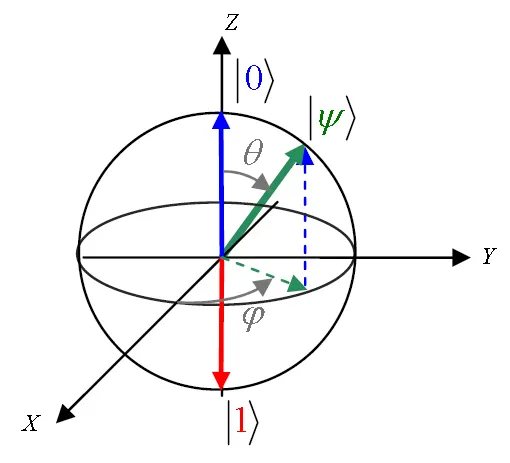
\includegraphics[width=0.5\linewidth]{imagenes/EsferaDeBloch.png}
    \caption{Visualización gráfica esfera de Bloch}
    \label{fig:EsferaDeBloch}
\end{figure}
\newpage

La representación de la esfera de Bloch de la imgaen, se le conoce como \textbf{ejes de Pauli}. Como tiene ángulos, se utiliza la representación de coordenadas esféricas principalmente. En dicha representación, se proporciona los dos ángulos y la longitud que viene denotado como $(r, \theta,\phi)$
donde $r$ es la longitud y $\theta$ y $\phi$ representan el ángulo del eje Z positivo con el de X positivo en el plano X-Z y el angulo entre el eje positivo X y el eje positivo Y del plano X-Y respectivamente
\end{comment}

\begin{figure}[h]
    \centering
    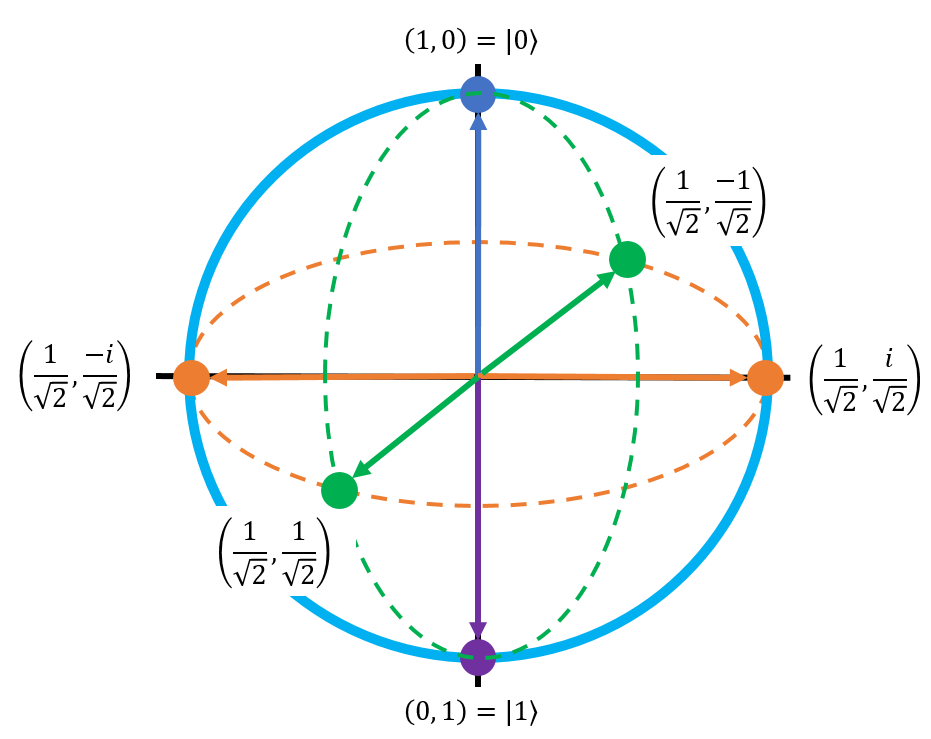
\includegraphics[width=0.5\linewidth]{imagenes/bloch-basic.png}
    \caption{Visualización gráfica de la esfera de Bloch. Imagen obtenida de \cite{mitre_bloch_sphere_2022}}
    \label{fig:EsferaDeBloch}
\end{figure}
\newpage

\textbf{Importante:} la notación $\left(\frac{1}{\sqrt{2}}, \frac{1}{\sqrt{2}}\right)$ se corresponde con el vector estado $\begin{bmatrix} \frac{1}{\sqrt{2}} \\ \frac{1}{\sqrt{2}} \end{bmatrix}$ que a su vez significa:

\[
    \begin{bmatrix} \frac{1}{\sqrt{2}} \\ \frac{1}{\sqrt{2}} \end{bmatrix} = \frac{1}{\sqrt{2}}|0\rangle + \frac{1}{\sqrt{2}}|1\rangle;
\]

Los seis puntos principales de la esfera de Bloch son los que se ve en la Figura \ref{fig:EsferaDeBloch} \cite{castano_qubit_bloch_2025}. A estas coordenadas principales se le pueden asignar etiquetas.

\begin{itemize}
    \item \textbf{Base de Hadamard:} También se le conoce como eje X de Pauli. El punto $\left(\frac{1}{\sqrt{2}}, \frac{1}{\sqrt{2}}\right)$ se corresponde con $\ket{+}$. A su vez, el punto opuesto $\left(\frac{1}{\sqrt{2}}, \frac{-1}{\sqrt{2}}\right)$ se corresponde con $\ket{-}$

    \item \textbf{Base circular:} También se le conoce como eje Y de Pauli. El punto $\left(\frac{1}{\sqrt{2}}, \frac{i}{\sqrt{2}}\right)$ se corresponde con $\ket{+i}$. A su vez, el punto opuesto $\left(\frac{1}{\sqrt{2}}, \frac{-i}{\sqrt{2}}\right)$ se corresponde con $\ket{-i}$
\end{itemize}

Con dicha asignación de etiquetas, queda la esfera que se muestra en la Figura \ref{fig:EsferaDeBlochReducido}:

\begin{figure}[h]
    \centering
    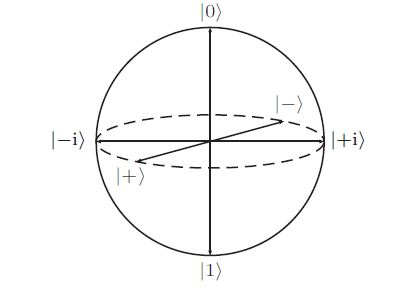
\includegraphics[width=0.5\linewidth]{imagenes/bloch-labels.jpg}
    \caption{Imagen obtenida de \url{https://en.wikipedia.org/wiki/Bloch_sphere}}
    \label{fig:EsferaDeBlochReducido}
\end{figure}
\newpage

\subsubsection{Puertas cuánticas}

Al igual que para manipular los valores de los bits existen puertas lógicas clásicas como OR, AND, NOT, etc. Los ordenadores cuánticos manipulan los valores de los qubits usando puertas cuánticas \cite{spinq_quantum_gates_2025}. Esto implica que cualquier algoritmo cuántico se tiene que implementar usando puertas cuánticas.

Las puertas cuánticas se \textbf{representan} matemáticamente mediante \textbf{matrices unitarias} $U$ \cite{gopalan_module3_2022}. Una matriz se considera unitaria si, al multiplicarla por su adjunta o conjugada transpuesta ($U^{\dagger}$), el resultado es la matriz identidad ($U^{\dagger}U = U U^{\dagger} = I$). Esta propiedad matemática es fundamental porque garantiza que la transformación es \textbf{reversible} y preserva la norma de los vectores. Esto significa que la puerta cuántica conserva siempre la probabilidad total de todos los posibles resultados, por lo que no se destruye ni se pierde información cuántica durante la operación.

Al aplicar una puerta cuántica $U$ a un estado cuántico $\ket{\psi}$ se realiza la multiplicación matricial $\ket{\psi'} = U \ket{\psi}$. Si expresamos el nuevo estado resultante como $\ket{\psi'} = \alpha_0' \ket{0} + \alpha_1' \ket{1}$, la propiedad unitaria asegura que la norma siga siendo unitaria. Es decir, independientemente de la puerta cuántica que se aplique, la regla de conservación de probabilidad se mantiene intacta: $|\alpha_0'|^2 + |\alpha_1'|^2 = 1$.

Poniendo un ejemplo sencillo, consideremos la puerta Pauli-X (el análogo cuántico de la puerta NOT clásica), cuya matriz unitaria es $X = \begin{pmatrix} 0 & 1 \\ 1 & 0 \end{pmatrix}$. Si aplicamos esta puerta sobre el estado base $\ket{0}$, el estado transiciona a $\ket{1}$:

\[
    X \ket{0} = \begin{pmatrix} 0 & 1 \\ 1 & 0 \end{pmatrix} \begin{pmatrix} 1 \\ 0 \end{pmatrix} = \begin{pmatrix} 0 \\ 1 \end{pmatrix} = \ket{1};
\]

Como $X$ es una matriz unitaria (y resulta ser su propia inversa, $X^{\dagger}X = I$), la operación es completamente reversible. Si aplicamos $X$ por segunda vez, recuperamos matemáticamente el estado original $\ket{0}$ sin perder ninguna información en el proceso:

\[
    X (X \ket{0}) = X \ket{1} = \begin{pmatrix} 0 & 1 \\ 1 & 0 \end{pmatrix} \begin{pmatrix} 0 \\ 1 \end{pmatrix} = \begin{pmatrix} 1 \\ 0 \end{pmatrix} = \ket{0};
\]

Las puertas cuánticas para un único qubit son:

\begin{itemize}
    \item \textbf{Pauli I (Identidad):} Se considera la operación trivial o identidad. Su función es dejar el qubit inalterado, y su operador asociado se denota mediante la matriz identidad $I$:
          \[
              I = \begin{bmatrix}
                  1 & 0 \\
                  0 & 1
              \end{bmatrix};
          \]

    \item \textbf{Pauli X:} Conocida coloquialmente como la puerta NOT cuántica. Algebraicamente se define por la siguiente matriz:
          \[
              X = \begin{bmatrix}
                  0 & 1 \\
                  1 & 0
              \end{bmatrix};
          \]

          Al aplicar esta puerta, las amplitudes de probabilidad se intercambian, lo que provoca que los estados base $\ket{0}$ y $\ket{1}$ se inviertan.

    \item \textbf{Pauli Y:} Esta transformación combina una inversión de los estados con un cambio de fase complejo. Su estructura viene dada por:
          \[
              Y = \begin{bmatrix}
                  0 & -i \\
                  i & 0
              \end{bmatrix};
          \]

          Si un qubit en superposición $\ket{\psi} = \alpha_0\ket{0} + \alpha_1\ket{1}$ atraviesa esta puerta, el efecto resultante es:
          \[
              Y\ket{\psi} = \begin{bmatrix} 0 & -i \\ i & 0 \end{bmatrix} \begin{bmatrix} \alpha_0 \\ \alpha_1 \end{bmatrix} = \begin{bmatrix} -i\alpha_1 \\ i\alpha_0 \end{bmatrix} = -i\alpha_1\ket{0} + i\alpha_0\ket{1};
          \]

    \item \textbf{Pauli Z:} Actúa modificando únicamente la fase del estado $\ket{1}$ (añadiendo un desfase de $\pi$). Su operador matricial se expresa como:
          \[
              Z = \begin{bmatrix}
                  1 & 0  \\
                  0 & -1
              \end{bmatrix};
          \]

          Matemáticamente, al operar sobre un qubit genérico $\ket{\psi} = \alpha_0\ket{0} + \alpha_1\ket{1}$, altera exclusivamente el signo de la segunda amplitud:
          \[
              Z\ket{\psi} = \begin{bmatrix} 1 & 0 \\ 0 & -1 \end{bmatrix} \begin{bmatrix} \alpha_0 \\ \alpha_1 \end{bmatrix} = \begin{bmatrix} \alpha_0 \\ -\alpha_1 \end{bmatrix} = \alpha_0\ket{0} - \alpha_1\ket{1};
          \]

    \item \textbf{Puerta Hadamard (H):} Es una de las operaciones más fundamentales, ya que al aplicarse sobre un estado base puro genera una superposición equitativa. Se define matricialmente como:
          \[
              H = \frac{1}{\sqrt{2}}\begin{bmatrix}
                  1 & 1  \\
                  1 & -1
              \end{bmatrix};
          \]

          Si aplicamos esta transformación a un estado en superposición $\ket{\psi} = \alpha_0\ket{0} + \alpha_1\ket{1}$, las amplitudes se mezclan obteniendo la siguiente salida:
          \[
              H\ket{\psi} = \frac{1}{\sqrt{2}}\begin{bmatrix} 1 & 1 \\ 1 & -1 \end{bmatrix} \begin{bmatrix} \alpha_0 \\ \alpha_1 \end{bmatrix} = \frac{1}{\sqrt{2}}\begin{bmatrix} \alpha_0 + \alpha_1 \\ \alpha_0 - \alpha_1 \end{bmatrix} = \left(\frac{\alpha_0 + \alpha_1}{\sqrt{2}}\right)\ket{0} + \left(\frac{\alpha_0 - \alpha_1}{\sqrt{2}}\right)\ket{1};
          \]
\end{itemize}


\subsection{Procesamiento del Lenguaje Natural Cuántico}
\label{chap:plnc}

El procesamiento de datos clásicos utilizando algoritmos de aprendizaje automático a través de sistemas cuánticos, ha generado una línea de investigación de especial foco de interés estos últimos años. El \gls{qml} se ha utilizado con distintos propósitos: profundizar en el uso de los fenómenos cuánticos para sistemas de aprendizaje, explorar la capacidad de los computadores cuánticos en aprender sobre datos cuánticos, y la posibilidad de reformular e implementar algoritmos de \gls{ml} en hardware cuántico.

Como ocurrió anteriormente en el caso del \gls{ml} clásico, el rápido crecimiento de los algoritmos de \gls{qml}, tanto desde el lado del hardware como del software (en términos de dispositivos y algoritmos), ha involucrado al campo de \gls{pln}. Esto ha dado lugar al llamado \gls{plnc}, definido como la implementación del procesamiento del lenguaje natural en hardware cuántico.

\subsubsection{Motivación para el uso de PLNC}

La investigación del \gls{plnc} está motivada fundamentalmente por las limitaciones físicas y computacionales de los modelos clásicos ante la creciente complejidad del lenguaje, especialmente tras la aparición de los \gls{llm}. Los sistemas tradicionales requieren recursos masivos de tiempo y memoria para procesar grandes conjuntos de datos (corpus, como por ejemplo la Wikipedia). Además, los modelos \gls{pln} clásicos sufren degradación en precisión y fiabilidad al enfrentarse por ejemplo a la polisemia, es decir, cuando una palabra tiene distintos significados según el contexto, debido a las restricciones de las arquitecturas clásicas (frecuentemente basadas en estructuras de árbol) \cite{guarasci_qnlp_2022}.

Para afrontar estos retos, el \gls{plnc} aprovecha fenómenos de la mecánica cuántica como la \textbf{superposición} y el \textbf{entrelazamiento}. Al operar en el espacio de \textit{Hilbert}, esta arquitectura permite almacenar múltiples significados y contextos simultáneamente en un solo registro y ejecutar operaciones en paralelo. Esto no solo ofrece una ventaja exponencial acelerando la computación \cite{qnlp_comp_survey}, sino que también proporciona una 'expresividad' superior, capturando las dependencias semánticas del lenguaje humano de una manera que los espacios numéricos clásicos replican con menor eficiencia.

No obstante, hay que tener en cuenta que, aunque teóricamente el \gls{plnc} puede resolver estos problemas, aún no se ha podido realizar una comparación a gran escala en hardware real (sin usar simuladores) frente a la computación clásica. Los modelos cuánticos actuales se han implementado sobre corpus pequeños, por lo que todavía no representan la escala completa que maneja un \gls{llm} moderno.

\subsubsection{Codificación de información clásica en estados cuánticos}

Una de las hipótesis fundamentales que motiva la intersección entre el procesamiento de lenguaje natural y la computación cuántica es la existencia de una relación estructural directa entre las características lingüísticas (sintáctica y semántica) y los estados cuánticos.

El framework \gls{discocat} \cite{wu2019categoricalcompositionaldistributionalmodelling} es el más conocido en formalizar esta relación. Nace de proponer la unificación de los dos enfoques clásicos del significado:
\begin{itemize}
  \item \textbf{Distribucional:} Basado en la estadística y el contexto, que es la base de los vectores de palabras modernos.
  \item \textbf{Composicional:} Basado en la estructura gramatical, donde el significado de una frase depende de sus partes y de cómo se combinan (reglas sintácticas).
\end{itemize}

La relevancia de DisCoCat para el \gls{plnc} radica en que modela el lenguaje utilizando diagramas de palabras y productos tensoriales, una estructura matemática que es a la que describe a su vez la computación cuántica. Esto sugiere que los ordenadores cuánticos son, de manera nativa, idóneos para procesar el lenguaje natural.

\begin{figure}[h]
  \centering
  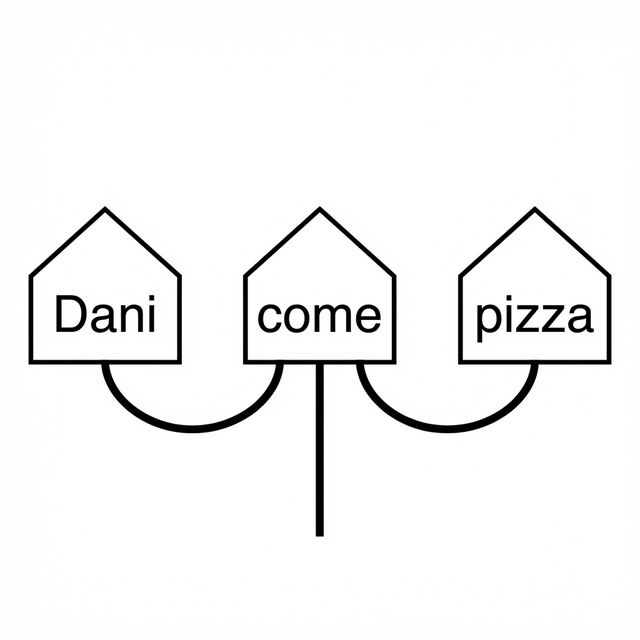
\includegraphics[width=0.4\linewidth]{imagenes/dani_come_pizza_discocat.png}
  \caption{Diagrama de la oración ``Dani come pizza'' en el formalismo DisCoCat.}
  \label{fig:DisCoCat_Dani}
\end{figure}

En la Figura \ref{fig:DisCoCat_Dani}, las cajas representan el significado de las palabras que se transmiten mediante los ``cables'', esto es similar a la técnica de \gls{dpt} muy popular en la literatura lingüística. En la frase, el sujeto es ``Dani'', mientras que ``pizza'' es el objeto, ambas palabras se relacionan mediante el verbo ``come'' y la combinación de estas palabras, crean el significado conjunto de la frase. Con DisCoCat, el significado de la oración se construye utilizando una gramática preagrupada mediante composición de productos tensoriales. Es decir, quedaría representado de la siguiente manera:

\[
  (\overrightarrow{\text{Dani}} \otimes \overrightarrow{\text{suj}}) \otimes \overrightarrow{\text{come}} \otimes (\overrightarrow{\text{pizza}} \otimes \overrightarrow{\text{obj}});
\]

En esta expresión matemática:
\begin{itemize}
  \item $\overrightarrow{\text{Dani}}$, $\overrightarrow{\text{come}}$ y $\overrightarrow{\text{pizza}}$ representan los vectores semánticos correspondientes a cada palabra individual.
  \item $\overrightarrow{\text{suj}}$ y $\overrightarrow{\text{obj}}$ son los vectores que codifican los roles sintácticos de sujeto y objeto, dictados por las reglas de la gramática.
  \item El operador $\otimes$ denota el producto tensorial, que es el mecanismo matemático que permite componer o entrelazar los significados léxicos con su función gramatical.
\end{itemize}

Todo este vector resultante generado en el espacio de productos tensoriales se puede considerar como el significado matemático de la oración completa ``Dani come pizza''. Por ende, se dice que este framework lo ha expresado en términos afines a la computación cuántica.

Cabe destacar que, aunque el modelo DisCoCat original funciona perfectamente sin referencias explícitas a la teoría cuántica (a pesar de originarse en el formalismo de la \gls{cqm}). La novedad yace en el argumento de que el \gls{plnc} puede considerarse ``nativo cuántico''. Esto se debe a que la teoría cuántica y el lenguaje natural comparten una misma estructura de interacción y el uso fundamental de espacios vectoriales para describir sus estados. Esta estructura de interacción determina por completo la estructura los procesos, incluyendo la especificación de los espacios donde ``viven'' los estados. Esta coincidencia estructural implica que el lenguaje natural podría encajar de manera más natural y eficiente en hardware cuántico que en hardware clásico.

\paragraph{Técnicas de codificación de datos clásicos a estados cuánticos}

Al igual que en computación clásica la información necesita ser codificada de manera que los modelos pueda entender los datos que se le proporcionan y así trabajar con ellos, la computación cuántica necesita poder codificar los datos de la computación clásica (texto en este caso, ya que estamos dentro del ámbito de \gls{pln} y \gls{plnc}), a estados cuánticos. Para ello existe diversas técnicas las cuales explicaremos a continuación:

\begin{itemize}
  \item \textbf{Basis Encoding:} Utiliza $n$ qubits. Complejidad $O(1)$. Simple, entradas cortas y simbólicas.
  \item \textbf{Angle Encoding:} Utiliza $n$ qubits. Complejidad $O(n)$. Resiliente al ruido, vectores de características pequeños.
  \item \textbf{Amplitude Encoding:} Utiliza $\log_2(n)$ qubits. Complejidad $O(2^n)$. Eficiente en memoria, vectores de frases completas.
  \item \textbf{Hamiltonian Encoding:} Utiliza $\log_2(n)$ qubits. Complejidad $O(t)$. Estructura de grafos, análisis sintáctico (parsing), traducción.
\end{itemize}

De todas estas técnicas, se ha optado por implementar la técnica de \textit{Basis Encoding} \cite{quantumzeitgeist_encoding_overview}. Este tipo de codificación se utiliza principalmente cuando un número real debe ser matemáticamente manipulado en un algoritmo cuántico. Su funcionamiento consiste en representar un número real como un número binario y luego transformarlo en un estado cuántico en la base computacional.

El estado cuántico embebido es la traducción bit a bit de una cadena binaria a los estados correspondientes de los subsistemas cuánticos. Por lo tanto, un bit de información clásica está representado por el estado de un subsistema cuántico. Actuar sobre características binarias codificadas como qubits otorga mayor flexibilidad computacional para diseñar algoritmos cuánticos.

Supongamos que queremos codificar la frase ``María estudia medicina'' utilizando \textit{Basis Encoding}. Primero, definimos un vocabulario simplificado donde asignamos un índice entero único a cada palabra y fijamos una longitud de $\tau = 5$ bits por palabra (lo que permitiría un vocabulario de hasta $2^5 = 32$ palabras).

\begin{itemize}
  \item \textit{María} $\rightarrow$ Índice 3 $\rightarrow$ \texttt{00011}
  \item \textit{estudia} $\rightarrow$ Índice 12 $\rightarrow$ \texttt{01100}
  \item \textit{medicina} $\rightarrow$ Índice 21 $\rightarrow$ \texttt{10101}
\end{itemize}

El vector de características de la frase corresponde entonces a la concatenación de estas secuencias binarias: $b = \texttt{00011 01100 10101}$.

Finalmente, esta secuencia se representa mediante el estado cuántico conjunto en la base computacional:

\[
  \ket{\psi}_{\text{frase}} = \ket{00011} \otimes \ket{01100} \otimes \ket{10101} = \ket{00011\;01100\;10101};
\]

De esta forma, hemos codificado una frase de lengua clásica directamente en un estado cuántico en la base computacional.

\subsubsection{Circuitos Variacionales Cuánticos como modelos de aprendizaje}

En 2016, se tuvo acceso al primer ordenador cuántico en la nube, aunque el ruido y las limitaciones
de quibits de las que se disponía hacía que fuera difícil implementar algoritmos cuánticos.

A pesar de estas limitaciones, se generó una gran expectación en la comunidad investigadora respecto al potencial que ofrecía esta nueva generación de dispositivos denominados \gls{nisq}. Estos ordenadores contaban con entre 50 y 100 \glsentryplural{qubit}, lo que les permitía superar en rendimiento a los mejores superordenadores clásicos en determinadas áreas matemáticas \cite{arute2019quantum,zhong2020quantum}.

Los \gls{cvc} nacieron como la mejor estrategia para hacer frente a los ordenadores \gls{nisq}. Debido a las limitaciones de estos dipsositivos, se utilizó la estrategia de optimización basado en el aprendizaje. No son más que una analogía cuántica a los técnicas existentes del campo de \gls{ml} como pueden ser las redes neuronales. En definitiva, son algoritmos cuánticos que tienen parámetros libres \cite{pennylane_variational_circuit}. Al igual que cualquier otro circuito cuántico estándar, se necesita hacer uso de estos tres conceptos básicos:

\begin{enumerate}
  \item Preparación con un \textbf{estado inicial} fijo.
  \item Un \textbf{circuito cuántico} $U(\theta)$ parametrizado con un conjunto de parámetros libres $\theta$.
  \item \textbf{Medición} de un observable $\hat{B}$ en la salida. Este observable puede estar compuesto por varios observables, cada uno de manera local a un cable del circuito, o bien, a un conjunto de cables del circuito.
\end{enumerate}

Para ilustrar estos tres conceptos de forma más intuitiva, imaginemos un sistema cuántico muy básico diseñado para clasificar el sentimiento de una frase (positivo o negativo):
\begin{itemize}
  \item \textbf{1. Preparación:} Se recibe la información de entrada (por ejemplo, la frase ``Me encanta'') y se codifica en el ordenador cuántico, alterando los qubits desde su estado base $\ket{0}$ hacia un estado que represente matemáticamente dicha frase.
  \item \textbf{2. Circuito parametrizado:} Actúa de forma análoga a las neuronas de una red neuronal clásica. Se aplican puertas lógicas cuánticas que dependen de unos ángulos $\theta$. Durante el entrenamiento, el algoritmo irá ajustando estos parámetros $\theta$ para aprender a separar las frases positivas de las negativas.
  \item \textbf{3. Medición:} Tras el circuito, se miden los qubits resultantes. Podemos definir por ejemplo que si el sistema colapsa mayoritariamente en el estado $\ket{0}$, el sentimiento predicho es ``positivo'', mientras que si colapsa en $\ket{1}$ es ``negativo''.
\end{itemize}

Normalmente, los valores esperados $f(\theta) = \langle 0 | U^\dagger(\theta) \hat{B} U(\theta) | 0 \rangle$ de uno o varios circuitos, definen un coste escalar para la tarea específica. Los parámetros libres $\theta = (\theta_1, \theta_2, \dots)$ son ajustados para optimizar esta función de coste, tal como se representa esquemáticamente en la Figura \ref{fig:costeVQC}: el circuito recibe los parámetros, aplica las transformaciones unitarias, obtiene un coste $f(\theta)$ mediante la medición del observable, y retroalimenta ese valor al optimizador clásico para actualizar $\theta$ en la siguiente iteración.

\begin{figure}[ht]
  \centering
  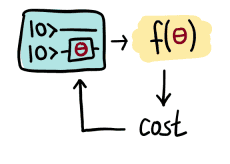
\includegraphics[scale=0.6]{imagenes/costeVQC.png}
  \caption{Coste de un Circuito Cuántico Variacional, imagen obtenida de: \cite{pennylane_variational_circuit}}
  \label{fig:costeVQC}
\end{figure}

Los circuitos cuánticos variacionales son entrenados mediante un algoritmo de optimización clásico que realiza consultas al hardware cuántico. La optimización suele ser un esquema iterativo que busca mejores candidatos para los parámetros en cada paso.

Los parámetros variacionales $\theta$, posiblemente junto con un conjunto adicional de parámetros no adaptables $x = (x_1, x_2, \dots)$, entran en el circuito cuántico como argumentos para las puertas del circuito. Esto nos permite convertir \textit{información clásica} (los valores $\theta$ y $x$) en \textit{información cuántica} (el estado cuántico $U(x; \theta)|0\rangle$). Como veremos en el ejemplo a continuación, los parámetros de puerta no adaptables suelen desempeñar el papel de \textit{entradas de datos} en el aprendizaje automático cuántico.

Finalmente, la información cuántica se convierte de nuevo en información clásica evaluando el valor esperado del observable $\hat{B}$, tal y como se esquematiza en la Figura \ref{fig:circuitoVQCArgumentos}:
\[
  f(x; \theta) = \langle \hat{B} \rangle = \bra{0} U^\dagger(x; \theta) \hat{B} U(x; \theta) \ket{0}.
\]
En esta expresión, $U(x; \theta)$ representa el circuito cuántico parametrizado que transforma el estado base $\ket{0}$: los parámetros $\theta$ son los pesos entrenables del modelo, mientras que $x$ son los datos de entrada no modificables (por ejemplo, la codificación cuántica de un texto). El operador $\hat{B}$ es el observable que se mide a la salida del circuito, y su valor esperado $\langle \hat{B} \rangle$ produce un escalar real que actúa como predicción del modelo para una tarea concreta (como la clasificación de sentimientos del ejemplo anterior).

\begin{figure}[htbp]
  \centering
  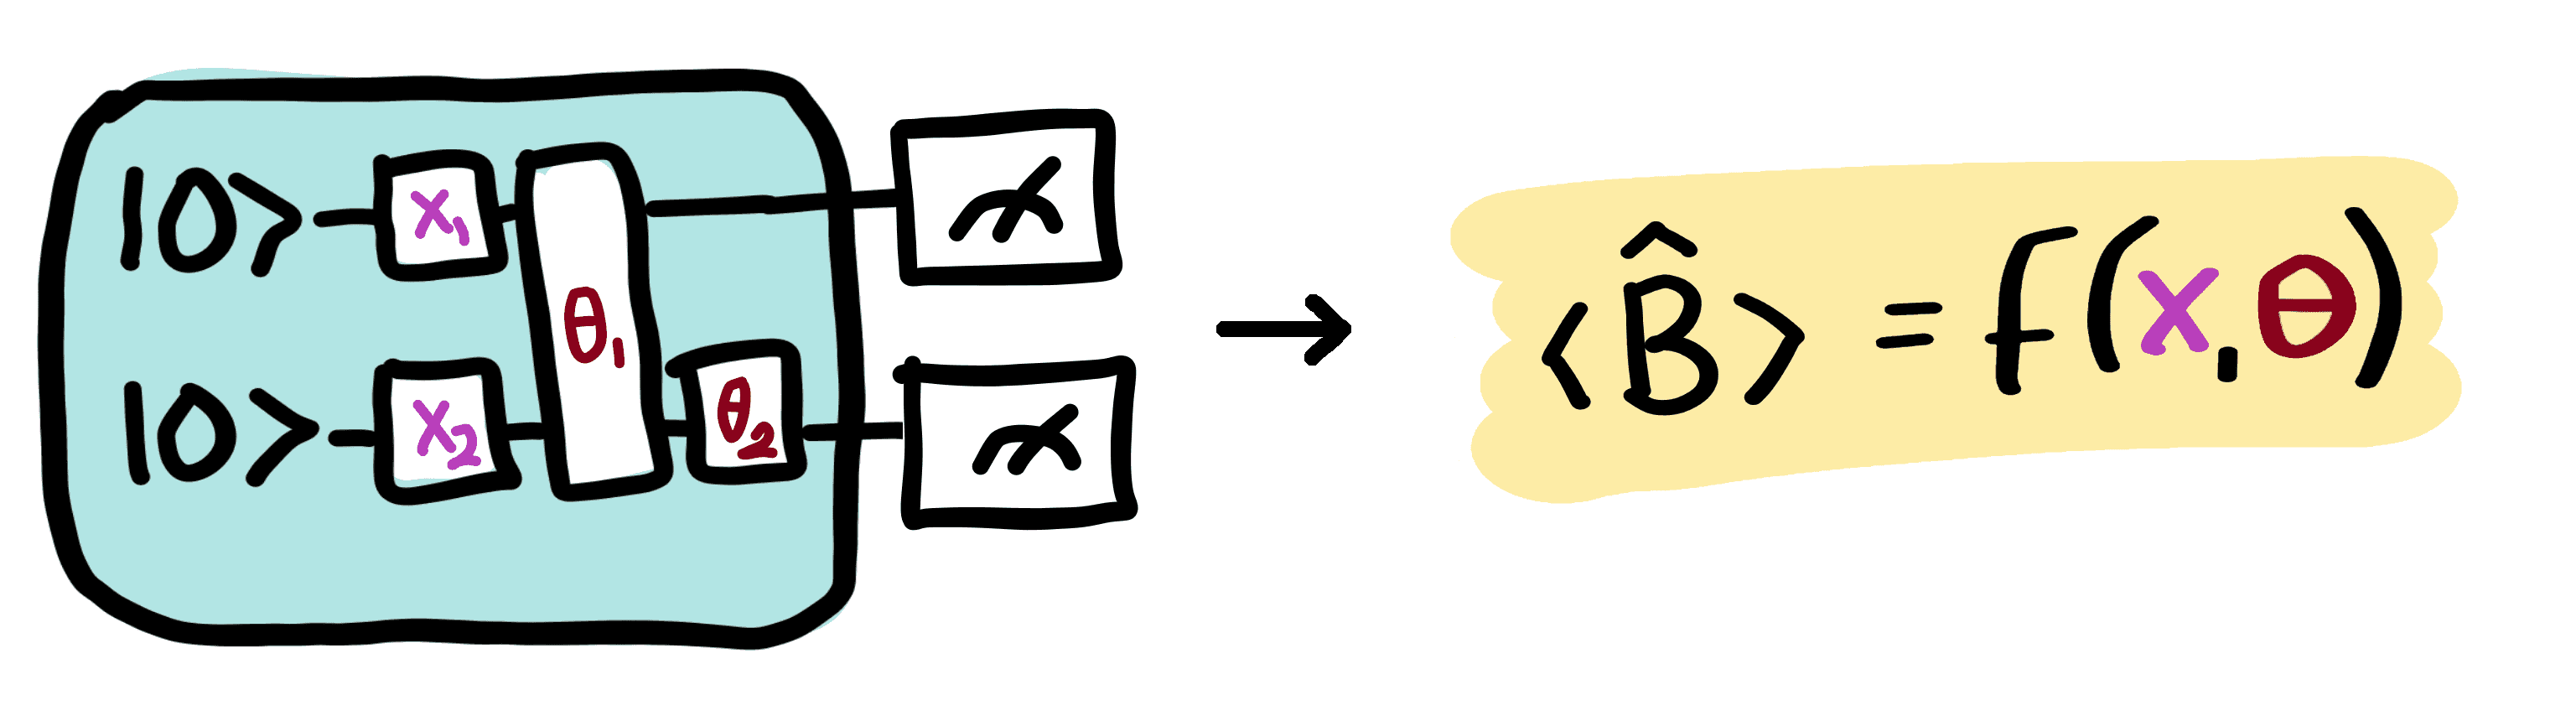
\includegraphics[scale=0.13]{imagenes/circuitoVQCArgumentos.png}
  \caption{Circuito variacional cuántico con parámetros modificables $x$ y no modificables $\theta$. Imagen obtenida de: \cite{pennylane_variational_circuit}}
  \label{fig:circuitoVQCArgumentos}
\end{figure}
